\question[6] 质量为$1.5\times 10^3kg$的汽车在水平路面上匀速行驶,速度为$20m/s$,受到的阻力大小为$1.8\times 10^3N.$此时,汽车发动机输出的实际功率是\key{C}
\fourchoices{$90W	$}{$30kW	$}{$36kW	$}{$300kW$}
\begin{solution}{4cm}

\end{solution}



\question[6] 电流互感器是一种测量电路中电流的变压器,工作原理如图所示。其原线圈匝数较少,串联在电路中,副线圈匝数较多,两端接在电流表上。则电流互感器\key{D}\begin{center}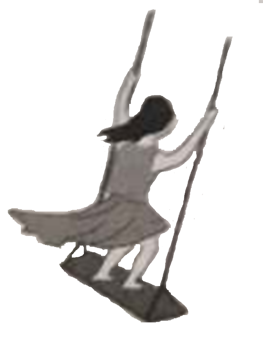
\includegraphics[]{img/image1.png}\end{center}
\fourchoices{是一种降压变压器	}{能测量直流电路的电流	}{原、副线圈电流的频率不同	}{副线圈的电流小于原线圈的电流}
\begin{solution}{4cm}

\end{solution}



\question[6] 如图所示,两匀强磁场的磁感应强度$B_1$和$B_2$大小相等、方向相反。金属圆环的直径与两磁场的边界重合。下列变化会在环中产生顺时针方向感应电流的是\key{B}\begin{center}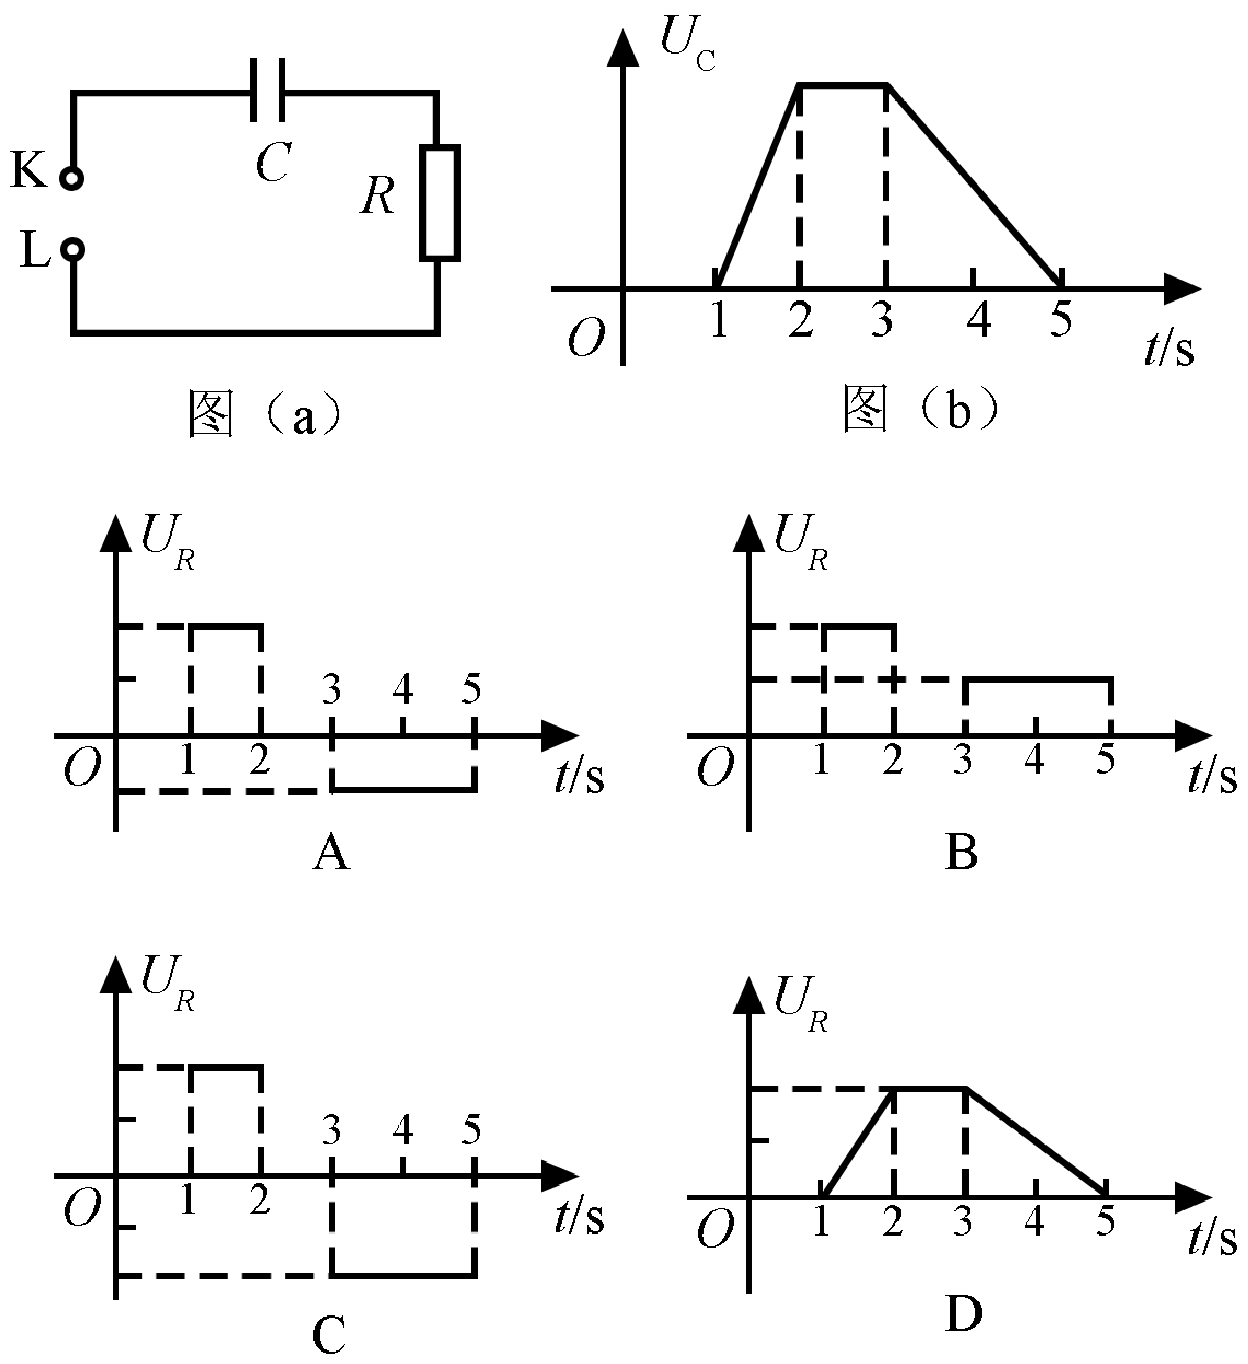
\includegraphics[]{img/image2.png}\end{center}
\fourchoices{同时增大$B_1$减小$B_2	$}{同时减小$B_1$增大$B_2	$}{同时以相同的变化率增大$B_1$和$B_2	$}{同时以相同的变化率减小$B_1$和$B_2$}
\begin{solution}{4cm}

\end{solution}


\newpage
\question[6] 如图所示,一小物块由静止开始沿斜面向下滑动,最后停在水平地面上。斜面和地面平滑连接,且物块与斜面、物块与地面间的动摩擦因数均为常数。该过程中,物块的动能$E_k$与水平位移x关系的图象是\key{A}
\begin{center}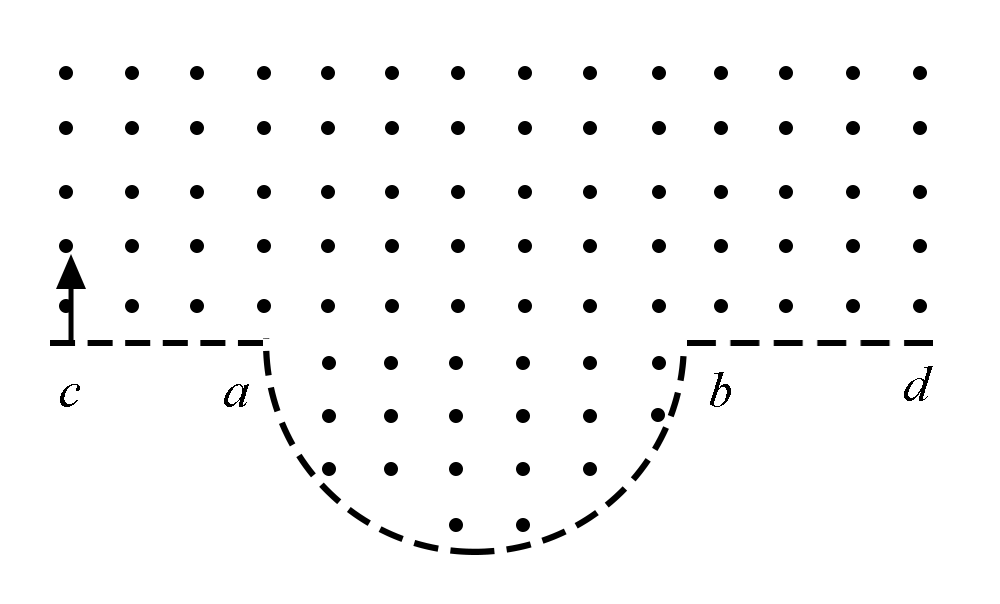
\includegraphics[width=5cm]{img/image3.png}\end{center}
\fourchoices{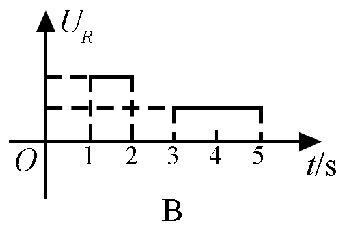
\includegraphics[]{img/image4.png}}{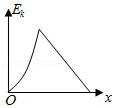
\includegraphics[]{img/image5.png}}{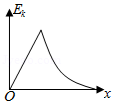
\includegraphics[]{img/image6.png}}{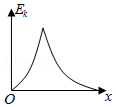
\includegraphics[]{img/image7.png}}
\begin{solution}{4cm}

\end{solution}



\question[6] 中欧班列在欧亚大陆开辟了“生命之路”,为国际抗疫贡献了中国力量。某运送防疫物资的班列由40节质量相等的车厢组成,在车头牵引下,列车沿平直轨道匀加速行驶时,第2节对第3节车厢的牵引力为F.若每节车厢所受摩擦力、空气阻力均相等,则倒数第3节对倒数第2节车厢的牵引力为\key{C}
\fourchoices{F	}{$\frac{19F}{20}	$}{$\frac{F}{19}	$}{$\frac{F}{20}$}
\begin{solution}{4cm}

\end{solution}

\end{questions}
\group{多项选择题}{本题共4小题,每小题4分,共计16分。每小题有多个选项符合题意。全部选对的得4分,选对但不全的得2分,错选或不答的得0分。}
\begin{questions}[30]

\question[6] 某汽车的电源与启动电机、车灯连接的简化电路如图所示。当汽车启动时,开关S闭合,电机工作,车灯突然变暗,此时\key{ABD}\begin{center}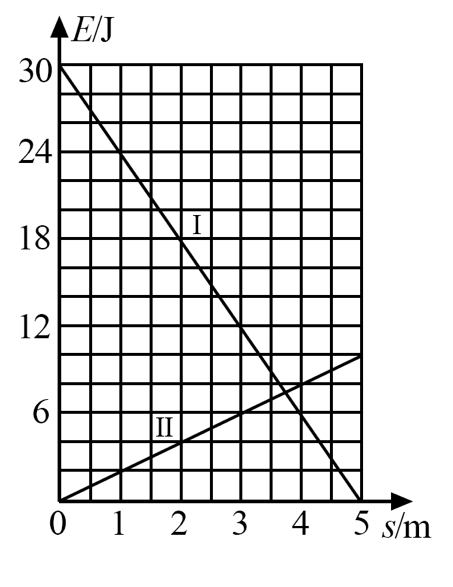
\includegraphics[width=4cm]{img/image8.png}\end{center}
\fourchoices{车灯的电流变小	}{路端电压变小	}{电路的总电流变小	}{电源的总功率变大}
\begin{solution}{4cm}

\end{solution}



\question[6] 甲、乙两颗人造卫星质量相等,均绕地球做圆周运动,甲的轨道半径是乙的2倍。下列应用公式进行的推论正确的有\key{CD}
\fourchoices{由$v=\sqrt{gR}$可知,甲的速度是乙的$\sqrt{2}$倍	}{由$a=\omega^{2}r$可知,甲的向心加速度是乙的2倍	}{由$F=G\frac{Mm}{r^{2}}$可知,甲的向心力是乙的$\frac{1}{4}$}{由$\frac{r^{3}}{T^{2}}=k$可知,甲的周期是乙的$2\sqrt{2}$倍}
\begin{solution}{4cm}

\end{solution}



\question[6] 如图所示,小球A、B分别从2l和l的高度水平抛出后落地,上述过程中A、B的水平位移分别为l和$21.$忽略空气阻力,则\key{AD}\begin{center}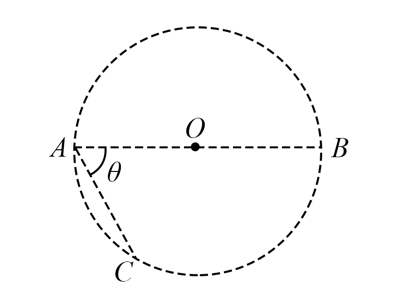
\includegraphics[]{img/image9.png}\end{center}
\fourchoices{A和B的位移大小相等	}{A的运动时间是B的2倍	}{A的初速度是B的$\frac{1}{2}	$}{A的末速度比B的大}
\begin{solution}{4cm}

\end{solution}



\question[6] 如图所示,绝缘轻杆的两端固定带有等量异号电荷的小球(不计重力)。开始时,两小球分别静止在A、B位置。现外加一匀强电场E,在静电力作用下,小球绕轻杆中点O转到水平位置。取O点的电势为0.下列说法正确的有\key{AB}\begin{center}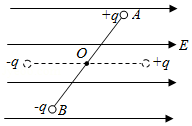
\includegraphics[]{img/image10.png}\end{center}
\fourchoices{电场E中A点电势低于B点	}{转动中两小球的电势能始终相等	}{该过程静电力对两小球均做负功	}{该过程两小球的总电势能增加}
\begin{solution}{4cm}

\end{solution}

\newpage

